\documentclass[12pt,a4paper]{article}

% Encoding og spraak
\usepackage[utf8]{inputenc}
\usepackage[T1]{fontenc}
\usepackage[nynorsk]{babel}

% Typografi
\usepackage{mathpazo}
\usepackage{microtype}

% Layout
\usepackage{geometry}
\geometry{a4paper, margin=2.5cm}
\usepackage{setspace}
\onehalfspacing

% Figurar og tabellar
\usepackage{graphicx}
\usepackage{float}
\usepackage{caption}
\usepackage{subcaption}
\usepackage{booktabs}
\usepackage{tabularx}

% Referansar (APA 7)

\usepackage[natbibapa]{apacite}
\usepackage{hyperref}
\hypersetup{
    colorlinks=true,
    linkcolor=black,
    citecolor=black,
    urlcolor=blue
}

% Diverse
\usepackage{csquotes}
\usepackage{amsmath}
\usepackage{enumitem}

% ---------------------------------------------
\title{Distribuert intelligens og fitnesslandskap:\\
\large Eit nytt paradigme for estetiske fag\\[0.5em]
\normalsize Kappe for ein PhD-serie om form, materialitet og industridesign}

\author{Iver Raknes Finne\\
\small Institutt for design, Arkitektur- og designh\o{}gskolen i Oslo (AHO)\\
\small\texttt{iver.raknes.finne@aho.stud.no}}

\date{Mars 2026}

\begin{document}
\maketitle

% ---------------------------------------------
\begin{abstract}
\noindent
I 130~\aa{}r har estetiske fag operert under eit deterministisk aksiom: \enquote{form follows function}. Denne kappa bind saman fire empiriske artiklar som til saman falsifiserer aksiomet og etablerer eit alternativ. Gjennom kvantitativ analyse av 461~stolar fr\aa{} Nasjonalmuseet (1280--2020), 401~tredimensjonale modellar og 740~\aa{}r med materialdata demonstrerer serien at: (1)~materialar er komprimerte geopolitiske historier der mahogniens boge avspeglar den transatlantiske kolonihandelen (Art.~I); (2)~stilmigrasjon f\o{}lgjer maktgeografiske linjer, ikkje formell logikk (Art.~II); (3)~rein 3D-geometri predikerer nasjon (76\,\% $F_1$) og stil (40{,}5\,\% $F_1$), medan funksjon forklarer ingenting (Art.~III); og (4)~material ber fem gonger meir informasjon om form enn geografi ($\mathrm{MI} = 0.382$ mot $0.079$), stilperiode er det d\aa{}rlegaste prediktoren av formklynger ($F_1 = 0.19$), og fitnesslandskapet skiftar dramatisk ved materialsjokk (Art.~IV). Kappa formulerer \emph{Form Follows Fitness} (FFF) som eit fullstendig paradigmeskifte: form er ikkje dedusert fr\aa{} funksjon, men selektert av eit fleirdimensjonalt fitnesslandskap der materialaffordanse, teknologi, \o{}konomi, geografi og kultur ut\o{}ver seleksjonstrykk. Sullivan og Le~Corbusier sine prinsipp er eit \emph{degenerert spesialtilfelle} av FFF, gyldig berre n\aa{}r alle seleksjonstrykk utanom funksjon er noytraliserte, eit vilk\aa{}r som aldri er oppfylt i praksis. Artikkelen viser at formgjeving er ein \emph{distribuert intelligent prosess} der materialet, verktyot, marknaden og kulturen alle ut\o{}ver agentur, parallelt med korleis slimsoppen \emph{Physarum} finn optimale baner utan hjerne. FFF gjer estetisk teori testbar, kvantifiserbar og operativ for designpraksis.

\medskip
\noindent\textbf{N\o{}kkelord:} form follows fitness, paradigmeskifte, distribuert intelligens, fitnesslandskap, seleksjonstrykk, materialaffordanse, designteori, estetiske fag
\end{abstract}

% ---------------------------------------------
\section{Innleiing: Ein revolusjon i fire akter}
\label{sec:innleiing}

Denne avhandlinga starta med eit enkelt eksperiment: \aa{} stille Sullivan sitt aksiom \enquote{form ever follows function} \citep{sullivan1896} p\aa{} pr\o{}ve mot eit reelt datasett. 461~stolar fr\aa{} Nasjonalmuseet, alle med same funksjon, alle m\aa{}lte, dokumenterte og modellerte. Dersom aksiomet heldt, burde formvariasjonen v\ae{}re liten. Ho var enorm.

Det som byrja som ein enkel test vart ei beviskjede p\aa{} fire ledd. Artikkel~I \citep{finne2026a} avdekte at materialar ikkje er n\o{}ytrale medium, men komprimerte geopolitiske historier. Artikkel~II \citep{finne2026b} viste at stilar migrerer langs maktgeografiske linjer, ikkje etter formell logikk. Artikkel~III \citep{finne2026c} demonstrerte at rein 3D-geometri kodar kulturell identitet og historisk tid. Artikkel~IV \citep{finne2026d} samla bevisa og formulerte \emph{Form Follows Fitness} (FFF) som eit koherent alternativ der form vert forst\aa{}tt som selektert av eit fleirdimensjonalt fitnesslandskap.

Denne kappa har tre oppg\aa{}ver: (1)~syntetisere beviskjeda til \'{e}i samanhengande forteljing, (2)~demonstrere at FFF eit fullstendig paradigmeskifte i Kuhn si tyding \citep{kuhn1962}, ikkje berre ein korreksjon, og (3)~vise at rammeverket generaliserer fr\aa{} stolar til alle estetiske fag.

% ---------------------------------------------
\section{Det gamle paradigmet}
\label{sec:gammalt}

\subsection{Sullivan, Le~Corbusier og det deterministiske aksiomet}

Louis Sullivan sin formulering fr\aa{} 1896, \enquote{form ever follows function}, var meint som ein poetisk observasjon av naturen \citep{sullivan1896}. Men etterf\o{}lgjande generasjonar gjorde han til eit \emph{aksiom}: ein udiskutabel premiss som heile designpedagogikken vart bygd p\aa{}. Le~Corbusier \citep{corbusier1923} radikaliserte premissen: huset er \enquote{une machine \`{a} habiter}, og kvar del m\aa{} tene ein funksjon. Loos \citep{loos1908} gjekk endaa lenger: ornament er kriminalitet.

Desse tre, Sullivan, Le~Corbusier og Loos, etablerte det me kan kalle \emph{det deterministiske aksiomet}: gjev ein funksjon, skal forma kunne \emph{deduserast}. Designaren sin jobb er \aa{} fjerne alt som ikkje tener funksjonen. Resultatet er \'{e}i optimal form. \citet{venturi1966} reagerte mot denne reduksjonismen med sitt \enquote{less is a bore}, men tilb\o{}d ikkje eit empirisk alternativ, berre ein estetisk motposisjon.

\subsection{Modulor: Universalitet som illusjon}

Le~Corbusier sitt Modulor-system \citep{corbusier1950} er den mest ambisi\o{}se konsekvensen av det deterministiske aksiomet: eit proposjonssystem basert p\aa{} den menneskelege kroppen, meint \aa{} gjelde universelt for all arkitektur og mekanikk. Premissen er at det finst \'{e}in optimal proporsjon derivert fr\aa{} funksjon (mennesket).

V\aa{}re data falsifiserer dette direkte. Blant 93~stolar med identisk funksjon varierer symmetri 15~gonger, djupn 3~gonger, og kompaktheit 2.6~gonger \citep{finne2026d}. Dersom \'{e}in universell proporsjon var optimal, burde variansen v\ae{}re null. Den er enorm. Modulor er ikkje feil fordi den er ein forenkling; den er feil fordi den er empirisk falsifisert.

\subsection{Alternativa som ikkje heldt}

Funksjonalismen har ikkje mangla kritikarar. \citet{pye1968} viste at form alltid er delvis kontingent, avhengig av materialets oppforsel og handverkaren sin dugleik. \citet{alexander1964} foreslo at form kan deriverast fr\aa{} ein dekomponering av designproblem, men aksepterte at resultatet er underdeterminert. Den postmoderne reaksjonen (Venturi, Jencks) avviste funksjonalismen, men erstatta han med relativisme: alle former er like gyldige. V\aa{}re data falsifiserer ogs\aa{} dette, fordi konvergensen i omsluttande volum \citep{finne2026b} viser at ikkje alle former er like fit.

\citet{simon1996} kom n\ae{}rast: design som s\o{}king i eit l\o{}ysingsrom. Men Simon mangla det evolusjon\ae{}re perspektivet, at l\o{}ysingsrommet sj\o{}lv endrar seg over tid, og at \enquote{s\o{}kinga} er distribuert, ikkje sentralisert. \citet{frazer1995} og \citet{steadman2008} brukte den biologiske analogien eksplisitt p\aa{} arkitektur og design, men typisk metaforisk, ikkje metrisk. FFF g\aa{}r fr\aa{} metafor til m\aa{}ling.

\subsection{Kvifor det gamle paradigmet overlevde}

\citet{kuhn1962} argumenterte for at vitskapelege paradigme ikkje fell fordi dei er motbevist, men fordi eit betre alternativ vert tilgjengeleg. \enquote{Form follows function} overlevde i 130~\aa{}r ikkje fordi det var korrekt, men fordi det var \emph{operativt}: det gav designstudentar eit enkelt prinsipp \aa{} arbeide etter. Problemet er at det er feil. Og no finst det eit betre alternativ.

% ---------------------------------------------
\section{Det nye paradigmet: Form Follows Fitness}
\label{sec:fff}

\subsection{Kjernepaastanden}

\emph{Form Follows Fitness} (FFF) seier: Forma p\aa{} eit objekt er ikkje dedusert fr\aa{} funksjonen, men \emph{selektert} av eit fleirdimensjonalt fitnesslandskap der kvar akse representerer eit seleksjonstrykk. Funksjon er eitt av desse trykka, og sjeldan det viktigaste.

Ideen om eit fitnesslandskap kjem fr\aa{} \citet{wright1932}: eit topografisk rom der kombinasjonar av variablar har ulik \enquote{fitness}. \citet{kauffman1993} generaliserte modellen til komplekse system og viste at n\aa{}r talet p\aa{} interagerande variablar aukar, vert landskapet meir ruglete, med fleire lokale optimum. I FFF er kvart slikt optimum ein \emph{stil}: ei mellombels stabil formkonfigurasjon som held s\aa{} lenge seleksjonstrykka held seg.

\subsection{Dei fem pilarane}

FFF kviler p\aa{} fem teoretiske pilarar:

\begin{enumerate}[nosep]
    \item \textbf{Fitnesslandskapet} \citep{wright1932, kauffman1993}: Form som posisjon i eit \emph{n}-dimensjonalt landskap. Stilar er lokale toppunkt.
    \item \textbf{Distribuert kognisjon} \citep{nakagaki2000, levin2019, clark2008}: Intelligens treng ikkje ein sentral styrar. Materialet \enquote{veit} kva det toler, verktyot avgrensar det moglege, marknaden selekterer det som overlever.
    \item \textbf{Exploration/exploitation} \citep{sutton2018, gould1972}: Designhistoria vekslar mellom utforsking av nytt terreng og utnytting av kjende optimum.
    \item \textbf{Affordanse} \citep{gibson1977, pye1968}: Kvart material tilbyr ei distinkt formverd, ikkje passivt men aktivt.
    \item \textbf{Morphospace} \citep{raup1966}: Rommet av alle moglege former, der faktiske objekt okkuperer avgrensa regionar.
\end{enumerate}

\subsection{Sullivan og Le~Corbusier som degenerert spesialtilfelle}

I FFF sin terminologi er \enquote{form follows function} gyldig \emph{berre} n\aa{}r alle seleksjonstrykk utanom funksjon er lik null:

\begin{equation}
\mathrm{MI_{material}} = \mathrm{MI_{tid}} = \mathrm{MI_{geografi}} = \mathrm{MI_{kultur}} = 0
\end{equation}

\noindent
V\aa{}re data viser at dette vilk\aa{}ret aldri er oppfylt. $\mathrm{MI_{material}} = 0.382$, $\mathrm{MI_{tid}} = 0.168$, $\mathrm{MI_{geografi}} = 0.079$ \citep{finne2026d}. Funksjon er per definisjon konstant ($\mathrm{MI_{funksjon}} = 0$, sidan alle objekta er stolar). Sullivan si lov er s\aa{}leis ikkje feil i absolutt forstand, men eit degenerert spesialtilfelle av ein meir generell dynamikk. Det er, i Kuhn sin terminologi, ein anomali som det gamle paradigmet ikkje kan forklare, og som det nye paradigmet subsumerer.

\subsection{Omgrepsapparatet}

Tabell~\ref{tab:omgrep} kartlegg det funksjonalistiske vokabularet over til FFF.

\begin{table}[H]
\centering
\caption{Fr\aa{} funksjonalisme til Form Follows Fitness: Omgrepsapparat}
\label{tab:omgrep}
\small
\begin{tabularx}{\textwidth}{p{2.8cm}p{2.8cm}X}
\toprule
\textbf{Gammalt omgrep} & \textbf{FFF-omgrep} & \textbf{Definisjon i FFF} \\
\midrule
Form follows function & Form follows fitness & Form er resultatet av eit fleirdimensjonalt fitnesslandskap, ikkje av funksjon \\
Funksjon & Seleksjonstrykk & Eitt av mange trykk: material, teknologi, \o{}konomi, kultur, funksjon \\
Designer & Distribuert agent & \'{E}in akt\o{}r i eit nettverk der materialet, verktyot og marknaden alle ut\o{}ver agentur \\
Material & Materialaffordanse & Materialet har ibuande agentur: det tilbyr og motset seg spesifikke former \\
Stil & Fitnessoptimum & Mellombels lokalt optimum i fitnesslandskapet \\
Stilendring & Exploration/exploitation & Veksling mellom utforsking og utnytting \\
Ornament & Kulturelt fitness-signal & Signal med reell seleksjonsverdi \\
Smak & Kulturell seleksjon & M\aa{}lbart, aggregert seleksjonstrykk \\
Formrom & Morphospace & Matematisk rom av alle moglege former \\
\bottomrule
\end{tabularx}
\end{table}

% ---------------------------------------------
\section{Beviskjeda: Fire artiklar, \'{e}in konklusjon}
\label{sec:bevis}

\subsection{Art.~I: Materialet som agent}

\citet{finne2026a} analyserte materialkurver for 461~stolar over 740~\aa{}r og avdekte \emph{mahogniens boge}: karibisk tropisk hardved stig fr\aa{} 0 til 93\,\% av norskproduserte stolar (1825--1849) og kollapsar deretter. Kurva f\o{}lgjer den transatlantiske mahognihandelen nesten synkront og plasserer museumsmagasinet som ein perifer node i eit kolonialt handelsnettverk.

\textbf{FFF-tolking}: Mahogni sin unike kombinasjon av h\o{}g brotstyrke, let bearbeidbarheit og kolonialt prestisjesignal skapte ein s\aa{} kraftig fitness-topp at heile det norske designlandskapet konvergerte, ein klassisk exploitation-syklus. Materialentropien kollapsa fr\aa{} 2.5 til 1.5~bit \citep{finne2026d}. Materialet er ikkje eit n\o{}ytralt medium; det er ein \emph{agent} med eigen affordanse \citep{gibson1977, ingold2007} som legg l\o{}ynde stiar i fitnesskartet.

\subsection{Art.~II: Kulturell seleksjon som distribuert intelligens}

\citet{finne2026b} kvantifiserer formevolusjon gjennom 3D-modellar av 289~stolar og avdekte \emph{fitness-konvergensen}: omsluttande volum konvergerer etter industrialiseringa, trass i aukande stilistisk divergens. Studien introduserte FFF-rammeverket og demonstrerte at Le~Corbusier sin maskinanalogi er falsifisert: form er ikkje determinert, men selektert.

\textbf{FFF-tolking}: Industrialiseringa innf\o{}rte nye seleksjonstrykk (masseproduksjon, transport, standardiserte rom) som eliminerte many tidlegare gyldige formar og skapte ein felles fitness-topp for volum. Samstundes diversifiserte materiale og stilar innanfor dette volumet, eit m\o{}nster som berre FFF kan forklare: konvergens i \'{e}in dimensjon (volum) med divergens i andre (form, material, estetikk).

\subsection{Art.~III: Form kodar identitet}

\citet{finne2026c} brukte maskinl\ae{}ring p\aa{} 401~tredimensjonale punktskyer og demonstrerte at rein geometri predikerer nasjon med 76\,\% $F_1$ og stil med 40{,}5\,\% $F_1$ \citep{breiman2001}. Funksjonen er invariant; forma er det ikkje. Form kodar kulturell identitet og historisk tid romleg og geometrisk.

\textbf{FFF-tolking}: Formrommet, visualisert gjennom UMAP som eit empirisk morphospace \citep{raup1966}, er ikkje tilfeldig utfylt. Stilperiodar okkuperer distinkte regionar, men med overlapp som reflekterer felles seleksjonstrykk. At kombinert geometri pluss material predikerer \emph{d\aa{}rlegare} enn material \'aleine demonstrerer materiell-formell kopling: redundansen \emph{er} koplinga.

\subsection{Art.~IV: Fitnesskartet}

\citet{finne2026d} la fram \aa{}tte empiriske bevis basert p\aa{} informasjonsteoretisk analyse av 93~stolar. Hovudfunna:

\begin{itemize}[nosep]
    \item Material ber fem gonger meir informasjon om form enn geografi ($\mathrm{MI} = 0.382$ mot $0.079$).
    \item Funksjon har $\mathrm{MI} = 0$ (per definisjon konstant).
    \item Stilperiode er det d\aa{}rlegaste prediktoren av formklynger ($F_1 = 0.19$).
    \item St\o{}rst drift i fitnesslandskapet ($11.7$ standardeiningar) samanfell med innf\o{}rsla av koloniale materiale.
    \item Materialentropi avspeglar exploration/exploitation: kollaps under mahognitoppen, ekspansjon under industrialiseringa.
\end{itemize}

\textbf{FFF-tolking}: Artikkelen demonstrerer FFF som \emph{operativt} rammeverk: dei \aa{}tte bevisa er ikkje isolerte funn, men manifestasjonar av same underliggjande dynamikk. Fitnesslandskapet er eit reelt, m\aa{}lbart terreng som forskuvar seg over tid, og forma f\o{}lgjer landskapet, ikkje funksjonen.

Det er verdt \aa{} dvele ved det mest oppsiktsvekkande funnet: \emph{stilperiode predikerer form d\aa{}rlegast av alle alternativ}. Berre stilperiode gjev $F_1 = 0.19$; berre tid gjev $F_1 = 0.44$; berre material gjev $F_1 = 0.33$. Stilkategoriane som designhistoria har brukt som forklaringsmodellar i eit hundre\aa{}r er, empirisk sett, dei svakaste forklaringane. Dei er symptom p\aa{} seleksjonstrykk, ikkje \aa{}rsaker til form. Denne konklusjonen er konsistent p\aa{} tvers av alle fire artiklane: Art.~I viser at materialkurver forklarer meir enn stilmerkelappar, Art.~II viser at fitness-konvergens kryssar stilgrenser, Art.~III viser at maskinl\ae{}ring predikerer stil betre fr\aa{} geometri enn fraa stilhistorisk intuisjon, og Art.~IV kvantifiserer denne asymmetrien presist.

\subsection{Den kumulative beviskjeda}

Dei fire artiklane dannar ein logisk sekvens (Tabell~\ref{tab:beviskjede}):

\begin{table}[H]
\centering
\caption{Beviskjeda: Fr\aa{} observasjon til paradigme}
\label{tab:beviskjede}
\small
\begin{tabularx}{\textwidth}{clX}
\toprule
\textbf{Art.} & \textbf{P\aa{}stand} & \textbf{Bevis} \\
\midrule
I & Material er ein formgjevande agent & Mahogniens boge, materiell dobbeltheit, 461 stolar \\
II & Form er selektert, ikkje dedusert & Fitness-konvergens i volum, falsifikasjon av Le~Corbusier \\
III & Form kodar identitet og tid & 3D-geometri predikerer nasjon (76\,\%) og stil (40{,}5\,\%) \\
IV & Fitnesslandskapet er reelt og m\aa{}lbart & MI-dekomponering, temporal drift, exploration/exploitation \\
\midrule
\textbf{Kappe} & \textbf{FFF er eit nytt paradigme} & \textbf{Syntese + generalisering til alle estetiske fag} \\
\bottomrule
\end{tabularx}
\end{table}

% ---------------------------------------------
\section{Generalisering: Fr\aa{} stolar til alle estetiske fag}
\label{sec:generalisering}

FFF er utvikla p\aa{} stolar, men mekanismane generaliserer. \citet{simon1996} argumenterte for at alle designproblem delar same struktur: s\o{}king i eit l\o{}ysingsrom under constraints. FFF presiserer dette: l\o{}ysingsrommet \emph{er} morphospace, constraints \emph{er} seleksjonstrykk, og den observerte designhistoria \emph{er} ei vandring gjennom fitnesslandskapet.

\begin{figure}[H]
    \centering
    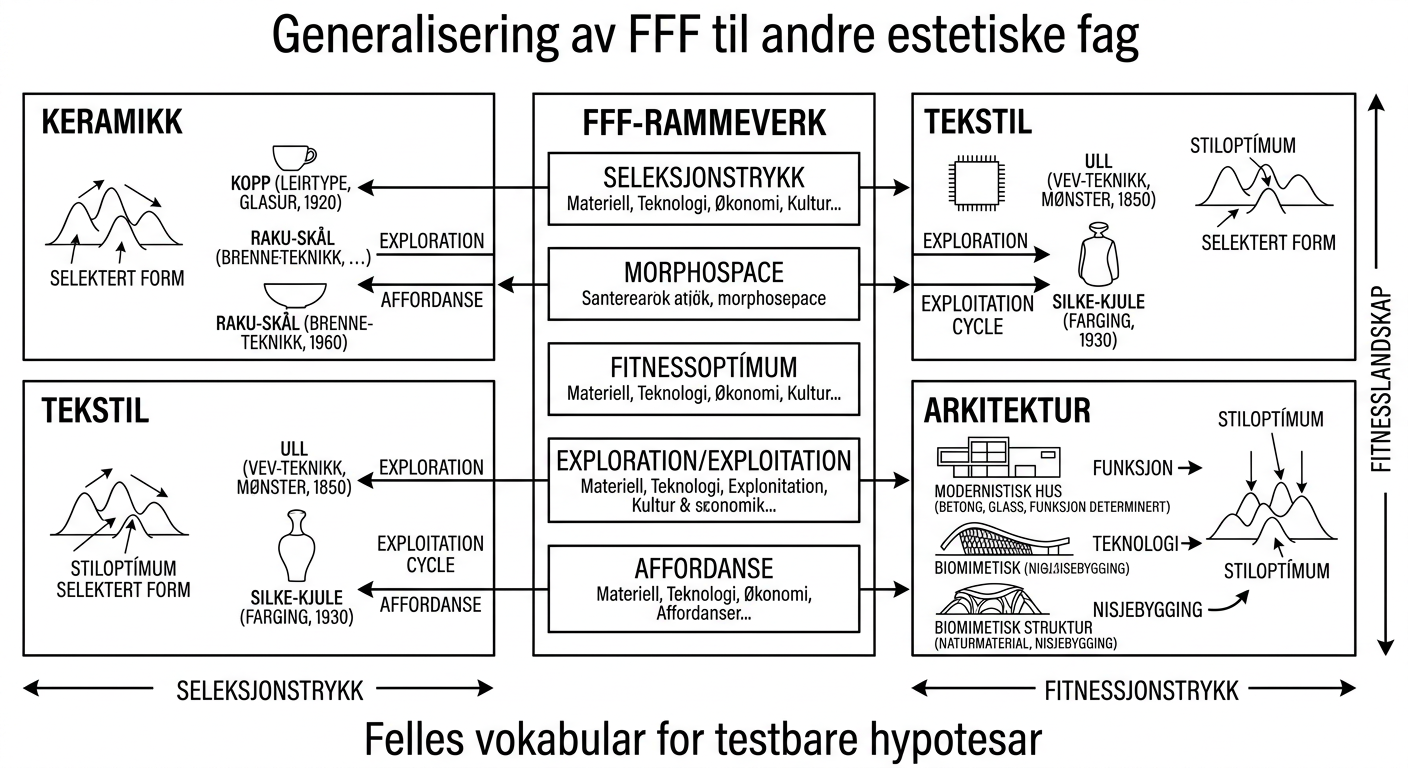
\includegraphics[width=0.8\textwidth]{figurar/fig2_fff_generalisering.png}
    \caption{Generalisering av FFF-rammeverket til keramikk, tekstil og arkitektur. Mekanismen er den same: form er selektert av eit fleirdimensjonalt landskap der material, teknologi, \o{}konomi og kultur ut\o{}ver trykk.}
    \label{fig:fff_generalisering}
\end{figure}

\subsection{Keramikk}

Ein kopp delar same funksjonelle invarians som ein stol: \aa{} halde v\ae{}ske. Men koppen sitt formrom er enormt. Glasur, leirtype, brennetemperatur og dreieskive ut\o{}ver alle seleksjonstrykk. I FFF-terminologi: glasuren er affordanse (som mahogni for stolen), tradisjonen er exploitation (som stilmigrasjon), og raku-teknikken er ein seleksjonsreset (som industrialiseringa).

\subsection{Tekstil}

Fiber, vev, farge og m\o{}nster definerer eit textile morphospace. Ull affordar andre former enn silke, p\aa{} same m\aa{}te som eik affordar andre stolear enn st\aa{}l. Motehistoria si exploration/exploitation-dynamikk, der trend\-syklusar vekslar mellom nyskaping og kopiering, er direkte analog til det me har m\aa{}lt i stoldata.

\subsection{Arkitektur}

\citet{norman2013} argumenterte for at god design handlar om \aa{} forst\aa{} affordansar. \citet{oxman2010} demonstrerte at materialbasert design\-tenking produserer former som er fundamentalt ulike dei funksjonsdeterminerte. I arkitektur er fitnesslandskapet endaa meir flerdimensjonalt: reguleringsplanar, materiallogistikk, klimatiske krav, kulturell kontekst og \o{}konomi ut\o{}ver alle trykk samstundes. Ingen av desse er reduserbare til \enquote{funksjon}.

\subsection{Det foreinande prinsippet}

Uavhengig av objekttype er mekanismen den same: form er selektert av eit fleirdimensjonalt landskap der material, teknologi, \o{}konomi og kultur ut\o{}ver trykk. Funksjon er eit hygienekrav, ikkje ein formgjevar.

\subsection{Eit felles vokabular}

FFF tilbyr eit \emph{felles vokabular} for alle estetiske fag: seleksjonstrykk, fitnesslandskap, morphospace, exploration/exploitation, affordanse. Dette vokabularet er presist nok til \aa{} v\ae{}re testbart og generelt nok til \aa{} gjelde for keramikk, glas, tekstil, arkitektur og industridesign.

Det som gjer FFF-vokabularet kraftigare enn det funksjonalistiske er at det er \emph{kompatibelt med kvantitative metodar}. \citet{manovich2020} demonstrerte at cultural analytics kan avdekke m\o{}nster i store kulturelle datasett. FFF gjev desse m\o{}nstra ein teoretisk struktur: dei er ikkje tilfeldige korrelasjonar, men manifestasjonar av seleksjonstrykk i fitnesslandskapet. Mutual information, PCA, Random Forest og Shannon-entropi er ikkje berre statistiske verktoy, dei er \emph{instrument for \aa{} lese fitnesskartet}. Kvar museumssamling i DigitaltMuseum, med sine tusenvis av digitaliserte objekt, er eit potensielt testbed for FFF. Kvar materialanalyse er ein MI-dekomponering. Kvar UMAP-projeksjon er eit morphospace. Rammeverket gjer kulturarvdata vitskapleg lesbare p\aa{} ein m\aa{}te som \enquote{form follows function} aldrig kunne.

% ---------------------------------------------
\section{Distribuert intelligens: Designaren som \'{e}in agent blant mange}
\label{sec:distribuert}

Det funksjonalistiske paradigmet set designaren i sentrum: \'{e}in intensjon, \'{e}in plan, \'{e}i optimal form. FFF snur dette p\aa{} hovudet.

\begin{figure}[H]
    \centering
    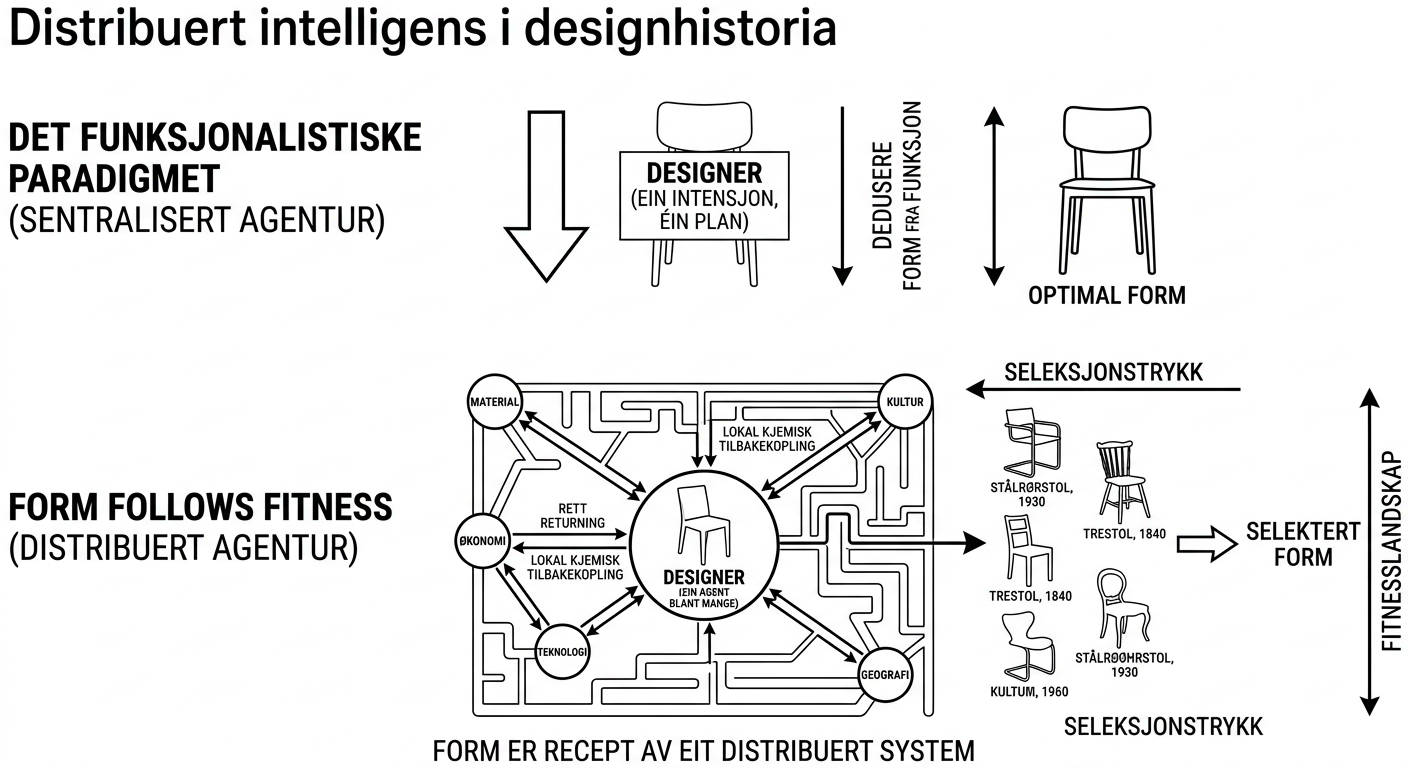
\includegraphics[width=0.8\textwidth]{figurar/fig1_distribuert_intelligens.png}
    \caption{Design som distribuert intelligent prosess. Intelligens er ikkje sentralisert i designaren, men spreidd over materialets affordanse, verktyets avgrensingar og marknadens seleksjon.}
    \label{fig:distribuert_intelligens}
\end{figure}

\subsection{Slimsoppen som modellorganisme}

\citet{nakagaki2000} viste at slimsoppen \emph{Physarum polycephalum} l\o{}yser labyrintar og optimaliserer nettverk utan hjerne, berre gjennom lokal kjemisk tilbakekopling. \citet{levin2019} generaliserte innsikta: kognitiv kapasitet, evna til \aa{} l\o{}yse problem og navigere mot m\aa{}l, eksisterer p\aa{} alle biologiske skalaer. Celler \enquote{veit} korleis dei skal organisere seg til organ; koloniar av insekt \enquote{veit} korleis dei skal byggje optimale strukturar.

\subsection{Designhistoria som distribuert prosess}

I FFF er formgjeving ein tilsvarande distribuert prosess \citep{hutchins1995, clark2008}:

\begin{itemize}[nosep]
    \item \textbf{Materialet} ut\o{}ver agentur gjennom sine fysiske eigenskapar. Mahogni \enquote{insisterer} p\aa{} slankare lemer; st\aa{}l \enquote{insisterer} p\aa{} rette linjer.
    \item \textbf{Verktyot} avgrensar det moglege. Dreieskiva produserer sirkel\ae{}re formar; CNC-fresen produserer frie kurver.
    \item \textbf{Marknaden} selekterer kva som overlever. Stolar som ikkje sel vert ikkje reproduserte.
    \item \textbf{Kulturen} premierer visse formar gjennom prestisje\-bias \citep{henrich2016} og costly signaling \citep{zahavi1975}.
    \item \textbf{Designaren} navigerer dette landskapet, les affordansane, og skapar variantar, men kontrollerer ikkje utfallet.
\end{itemize}

\noindent
Designaren er ikkje ein eineveldig skapar, men \'{e}in agent i eit distribuert system. Forma som kjem ut er ikkje \'{e}in person sin intensjon, men eit \emph{emergent resultat} av many samverkande seleksjonstrykk, nett slik slimsoppen sitt optimale nettverk er eit emergent resultat av many samverkande celler.

\subsection{Nisjebygging}

\citet{odlingsmee2003} viste at organismar ikkje berre tilpassar seg milj\o{}, men aktivt modifiserer det. Stolar gjer det same: ein stol designa for eit kontor endrar sitjevanar, som endrar kva som tel som \enquote{fit} for neste generasjon kontorstolar. Designobjekt konstruerer si eiga nisje. Fitnesslandskapet er ikkje ein ekstern realitet designaren tilpassar seg, det er ein dynamisk overflate som designaren samskaper med materialet, marknaden og kulturen.

% ---------------------------------------------
\section{FFF som pedagogisk rammeverk}
\label{sec:pedagogikk}

Dersom FFF erstattar \enquote{form follows function} som grunnleggande prinsipp, endrar det korleis me underviser i estetiske fag.

\subsection{Fr\aa{} funksjonskravsdokument til seleksjonstrykk-kartlegging}

I staden for \aa{} starte designprosessen med sp\o{}rsm\aa{}let \enquote{kva er funksjonen?}, b\o{}r studenten starte med: \enquote{kva er seleksjonstrykka?} Materialtilgang, produksjonsmetode, \o{}konomiske vilk\aa{}r, kulturell kontekst, berekraft, ergonomi, og ja, funksjon, men som \'{e}itt trykk blant mange. Fitnesskartet vert designverkt\o{}yet.

\subsection{Materialval som prim\ae{}r designvariabel}

V\aa{}re data viser at material er det st\o{}rste einskildtrykket ($\mathrm{MI} = 0.382$). Designprosessen b\o{}r starte med materialets affordanse \citep{gibson1977, oxman2010}, ikkje med ei skisse p\aa{} eit blankt ark. \citet{pye1968} visste dette intuitivt; FFF stadfestar det kvantitativt.

\subsection{Stilkategoriar som diagnostikk, ikkje m\aa{}l}

\AA{} designe \enquote{i ein stil} er \aa{} kopiere eit symptom utan \aa{} forst\aa{} \aa{}rsaka. V\aa{}re data viser at stilperiode er det d\aa{}rlegaste prediktoren av form ($F_1 = 0.19$). Stilkategoriar er nyttige som \emph{diagnostiske verkty}, dei fortel kva seleksjonstrykk som var operative, men d\aa{}rlege som \emph{designm\aa{}l}.

\subsection{Evolution\ae{}r lesekompetanse}

FFF krev ein ny type lesekompetanse i designfaga. Studenten m\aa{} kunne lese eit objekt ikkje berre estetisk, men evolusjon\ae{}rt: Kva seleksjonstrykk produserte denne forma? Kva fitness-topp okkuperer objektet? Kva endringar i landskapet ville gjort forma ufit? Denne kompetansen er analog til Darwin sin evolusjon\ae{}re lesekompetanse \citep{darwin1859, dennett1995}: evna til \aa{} sj\aa{} design overalt der det er seleksjon, utan \aa{} anta ein designar.

% ---------------------------------------------
\section{FFF som vitskapsteori: Paradigmeskiftet}
\label{sec:paradigme}

\citet{kuhn1962} identifiserte fire kjenneteikn p\aa{} eit paradigmeskifte: (1)~akkumulering av anomaliar som det gamle paradigmet ikkje kan forklare, (2)~ein kriseperiode der anomaliane vert uignorlege, (3)~formuleringa av eit nytt paradigme som l\o{}yser anomaliane, og (4)~at det nye paradigmet subsumerer det gamle som spesialtilfelle.

FFF oppfyller alle fire:

\begin{enumerate}[nosep]
    \item \textbf{Anomaliar}: 15$\times$ variasjon i symmetri blant objekt med identisk funksjon. Stilperiode som d\aa{}rlegaste prediktor av form. Material som den st\o{}rste formgjevaren.
    \item \textbf{Krise}: 130~\aa{}r utan empirisk testing av det deterministiske aksiomet. Postmodernismen reagerte, men tilb\o{}d ikkje eit alternativ, berre ein negasjon.
    \item \textbf{Nytt paradigme}: FFF formulerer form som selektert av eit fleirdimensjonalt fitnesslandskap, med presist vokabular og testbare prediksjonar.
    \item \textbf{Subsumering}: Sullivan er eit degenerert spesialtilfelle der alle MI utanom funksjon er null (ligning~1).
\end{enumerate}

\begin{figure}[H]
    \centering
    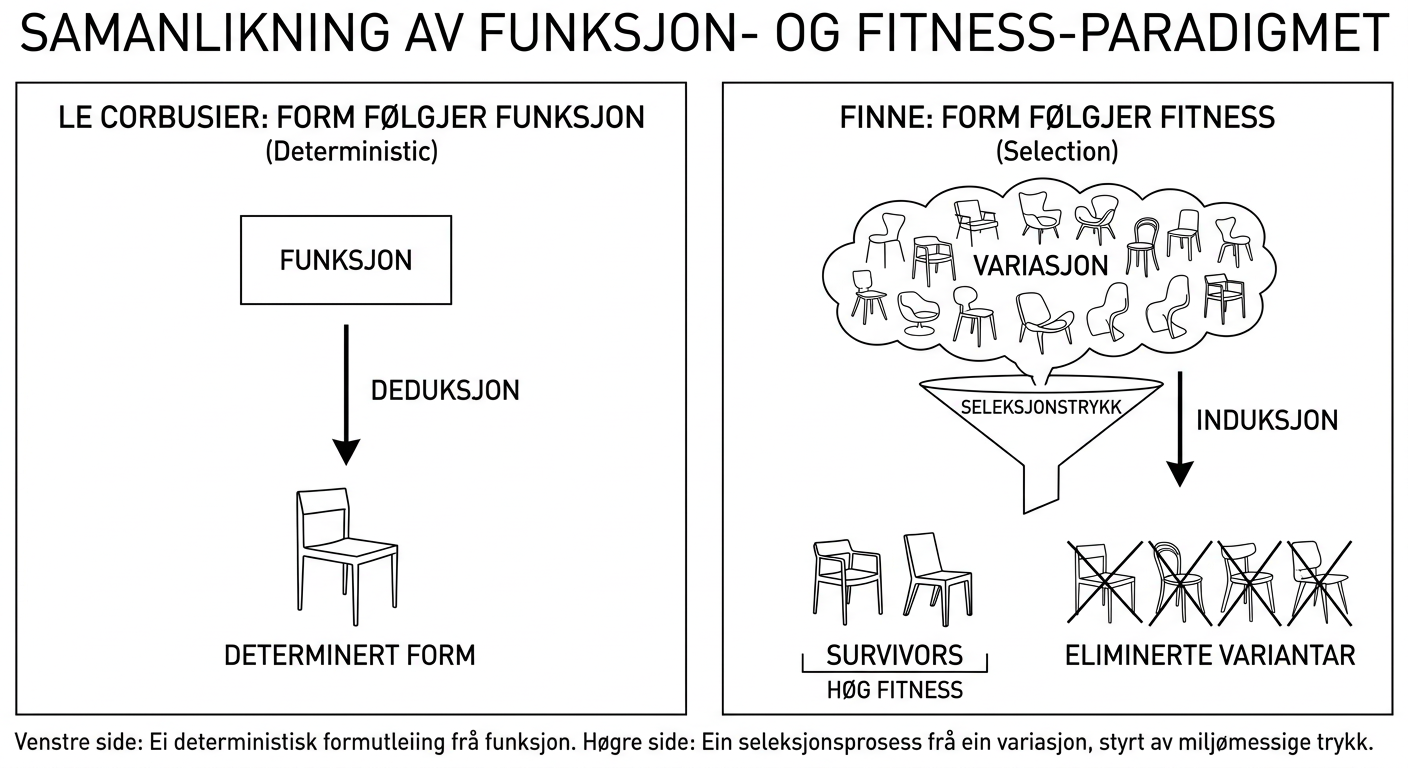
\includegraphics[width=0.9\textwidth]{figurar/fig3_samanlikning_paradigme.png}
    \caption{Paradigmeskiftet: Fr\aa{} deterministisk funksjonalisme til evolusjon\ae{}r FFF. FFF subsumerer Sullivan og Le Corbusier som eit degenerert spesialtilfelle der alle seleksjonstrykk utanom funksjon er noytraliserte.}
    \label{fig:paradigmeskifte}
\end{figure}

\noindent
Det nye paradigmet er ikkje berre ein \emph{betre} teori. Det er ein teori av ein annan type: empirisk der den gamle var aksiomatisk, kvantitativ der den gamle var kvalitativ, distribuert der den gamle var sentralisert. Og viktigast: falsifiserbar. Kvar ny museumssamling, kvar ny objekttype, kvar ny MI-analyse kan potensielt motbevise FFF. Det kunne aldri \enquote{form follows function}, fordi aksiomet aldri var formulert presist nok til \aa{} v\ae{}re falsifiserbart.

% ---------------------------------------------
\section{Avgrensingar og framtidig forsking}
\label{sec:avgrensingar}

\subsection{Avgrensingar}

Beviskjeda har klare avgrensingar: (1)~\'{e}i samling fr\aa{} \'{e}itt museum; (2)~\'{e}in objekttype (stolar); (3)~museumsseleksjonsskaevheit (prestisje\-objekt overrepresentert); (4)~handlaga geometriske features, ikkje end-to-end deep learning; (5)~$n = 93$ med komplett data for MI-analysen i Art.~IV; (6)~dateringane er i many tilfelle estimat. Trass i desse avgrensingane er beviskjeda kumulativ: kvar artikkel brukar ulike metodar p\aa{} ulike delsett av same samling, og konklusjonane konvergerer.

\subsection{Framtidig forsking}

FFF opnar fem forskingslinjer:

\begin{enumerate}[nosep]
    \item \textbf{Kryssmuseum-validering}: Teste FFF p\aa{} samlingar fr\aa{} Victoria \& Albert Museum, MoMA, Designmuseum Danmark.
    \item \textbf{Kryssobjekt-validering}: Teste FFF p\aa{} keramikk, glas, tekstil og industriprodukt fr\aa{} DigitaltMuseum.
    \item \textbf{Deep learning}: Erstatte handlaga features med PointNet/DGCNN for end-to-end formanalyse.
    \item \textbf{Generativt fitnesskart}: Bruke fitnesslandskapet som input til generative designverktoy.
    \item \textbf{Temporell regresjon}: Predikere \aa{}rstal fr\aa{} form, ein kvantitativ test p\aa{} kor mykje historisk informasjon geometrien ber.
\end{enumerate}

% ---------------------------------------------
\section{Konklusjon}
\label{sec:konklusjon}

461~stolar. 401~tredimensjonale modellar. 740~\aa{}r med data. Fire artiklar. \'{E}in konklusjon:

\emph{Form follows fitness.}

Beviskjeda er kumulativ og konvergent. Materialar er ikkje n\o{}ytrale medium, men agentar med eigen affordanse (Art.~I). Stilar migrerer langs maktgeografiske linjer, ikkje etter formell logikk (Art.~II). Form kodar kulturell identitet og historisk tid in 3D-geometri (Art.~III). Fitnesslandskapet er reelt, m\aa{}lbart og dynamisk, med material som det st\o{}rste seleksjonstrykket og funksjon som det minste (Art.~IV).

Sullivan sitt \enquote{form follows function} er ikkje ein feil. Det er eit \emph{degenerert spesialtilfelle} av ein meir generell dynamikk, gyldig berre n\aa{}r alle seleksjonstrykk utanom funksjon er lik null. Eit vilk\aa{}r som aldri er oppfylt. Le~Corbusier sin Modulor er ikkje universell; den er falsifisert av 15~gonger variasjon i symmetri blant objekt med identisk funksjon.

Formgjeving er ikkje ein deterministisk prosess styrt av \'{e}in intensjon. Det er ein \emph{distribuert intelligent prosess} der materialet, verktyot, marknaden og kulturen alle ut\o{}ver agentur, lik slimsoppen som finn optimale baner utan hjerne.

\emph{Form Follows Fitness} gjer estetisk teori det den aldri har vore: \textbf{testbar}. Kvantifiserbar. Falsifiserbar. Operativ. Rammeverket er ikkje ein filosofisk posisjon, men ein empirisk modell, open for testing p\aa{} kvar museumssamling i verda, utvidbar til kvart designobjekt, og anvendbar i kvar designstudio.

Fitnesskartet erstattar aksiomet. Verktyet erstattar dogmet.

% ---------------------------------------------
\bibliographystyle{apacite}
\bibliography{referansar}

\end{document}
